\documentclass[aspectratio=169, 10pt]{beamer}

\usetheme{simear}

\title{Title of Presentation Here}
\subtitle{Subtitle Here}
\author{Author Here}
\date{\today}

\begin{document}

\begin{frame}[plain]
\titlepage
\end{frame}

\begin{frame}{Bullets}
  \begin{itemize}
    \item Item 1
    \item {
        Item 2
        \begin{itemize}
            \item Subitem 1
            \item {
                Subitem 2
                \begin{itemize}
                    \item Subsubitem 1
                    \item Subsubitem 2
                \end{itemize}
            }
            \item Subitem 3
        \end{itemize}
    }
    \item Item 3
  \end{itemize}
\end{frame}

\begin{frame}{Columns}
    \begin{columns}[t]
        \begin{column}{0.5\textwidth}
            \begin{itemize}
                \item This is text for Item 1
                \item And this is text for Item 2
            \end{itemize}
        \end{column}

        \begin{column}{0.5\textwidth}
            \begin{figure}
                \centering
                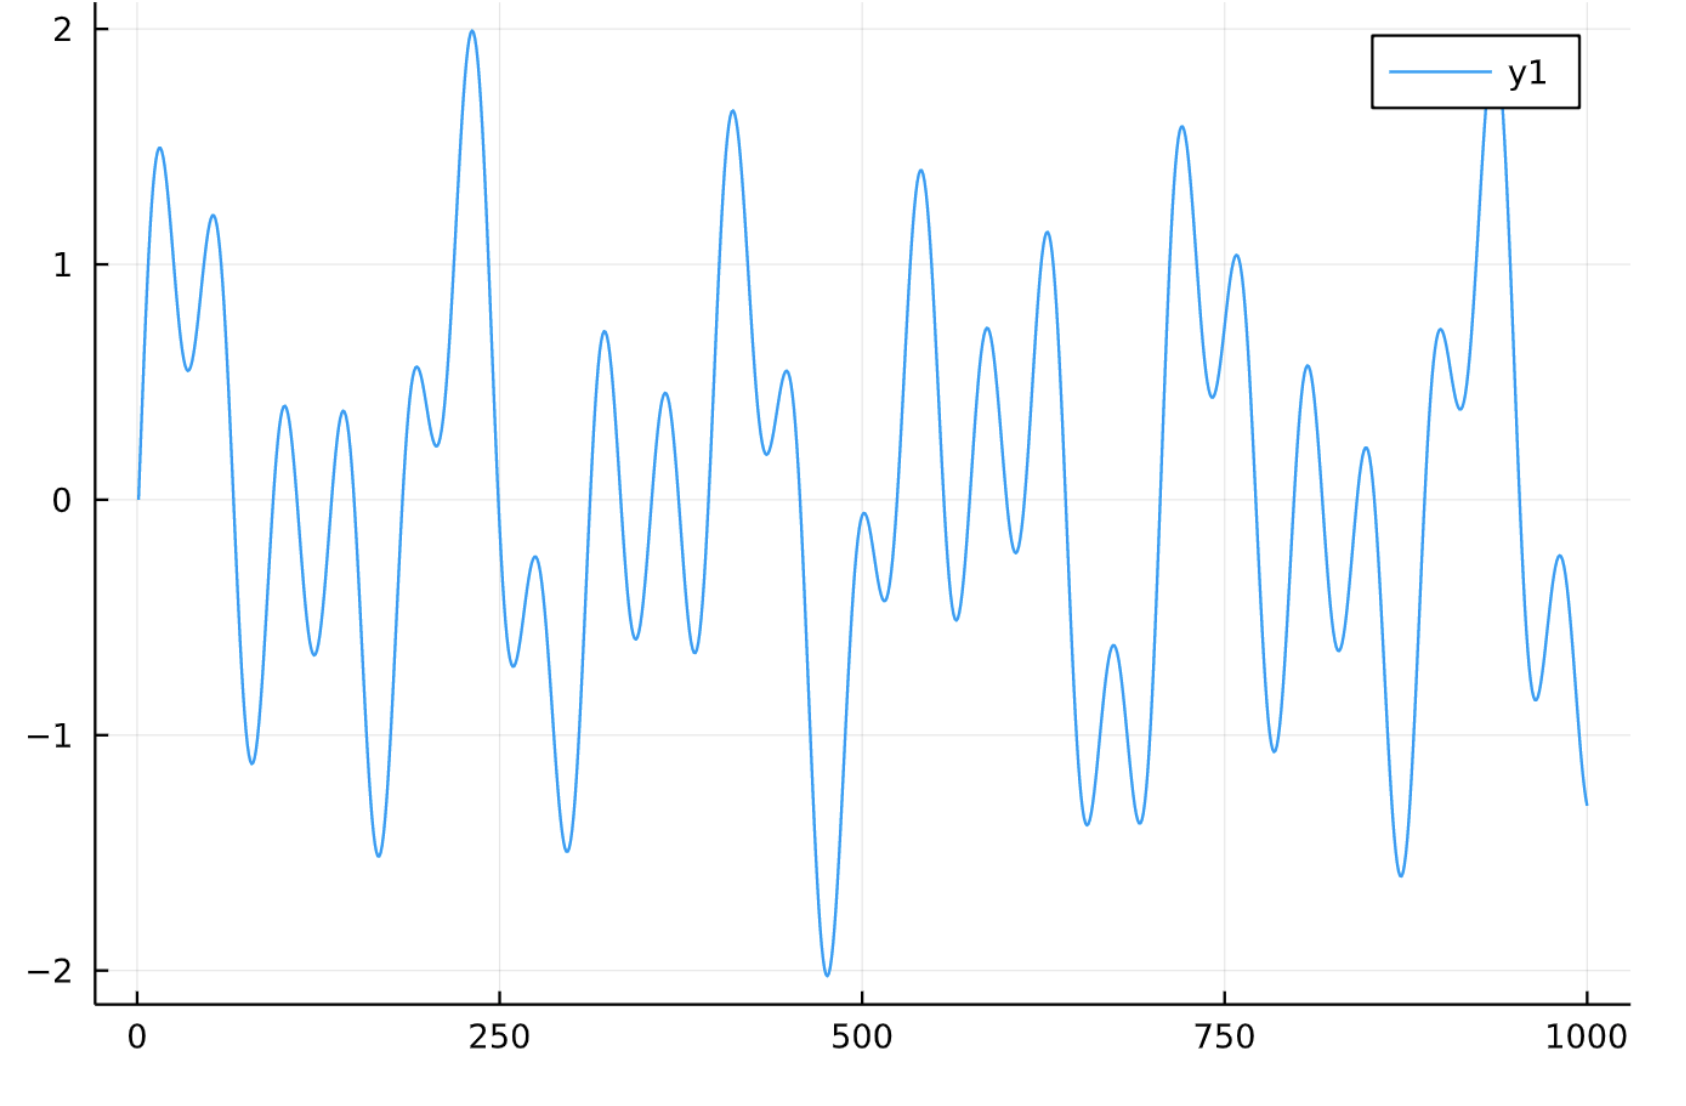
\includegraphics[width=\textwidth]{
                    assets/slides/image-1.png
                }
                \caption{A caption}
                \label{fig:figure-a}
            \end{figure}
        \end{column}
  \end{columns}
\end{frame}

\begin{frame}{Figures}
    \begin{figure}
        \centering
        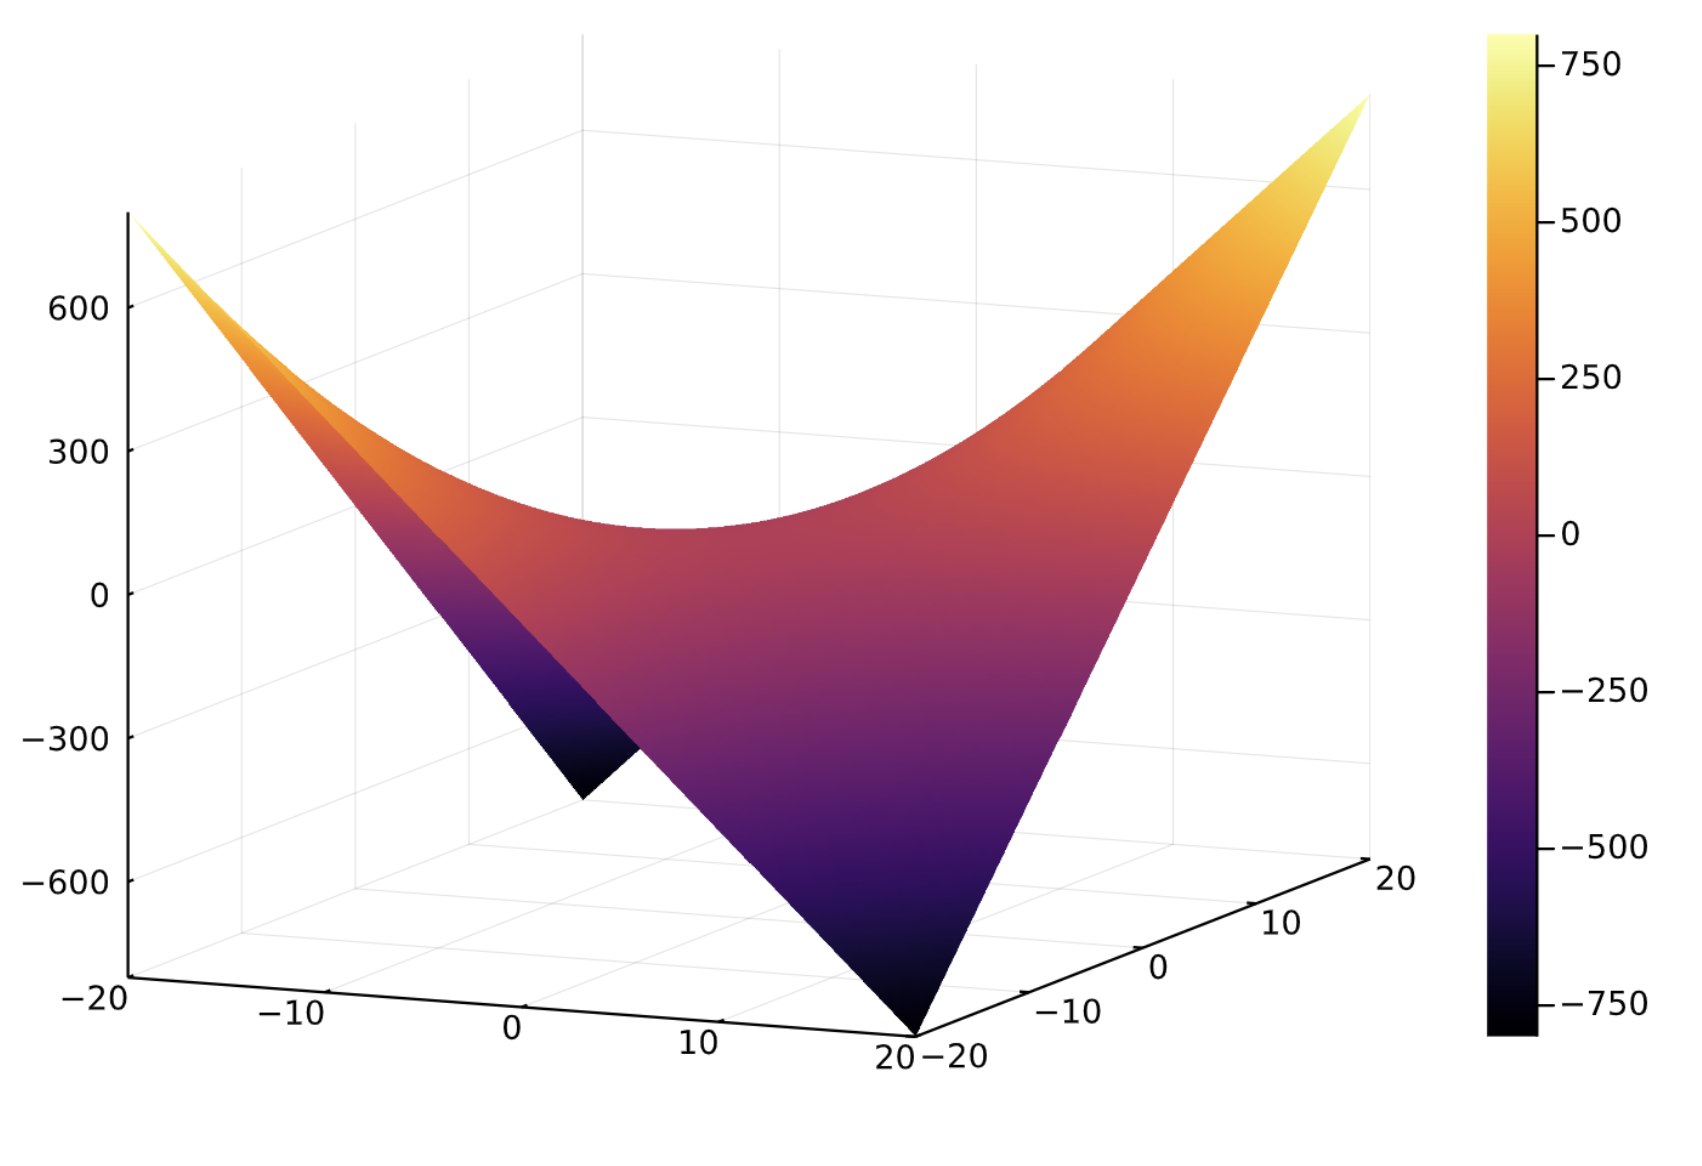
\includegraphics[width=0.5\textwidth]{
            assets/slides/image-2.png
        }
        \caption{This is a caption for the figure}
        \label{fig:figure-b}
    \end{figure}
\end{frame}

\begin{frame}{Blocks}
  \begin{block}{Regular block}
    This is a regular block
  \end{block}
  
  \begin{exampleblock}{Example block}
    This is an example block
  \end{exampleblock}

  \begin{alertblock}{Alert block}
    This is an alert block
  \end{alertblock}

  \begin{definition}
    This is a definition block
  \end{definition}
\end{frame}

\begin{frame}[fragile]{Code}
\begin{lstlisting}[frame=single,language=Haskell, numbers=left]
-- This is some code

main = do
  putStrLn "Hello, world"
\end{lstlisting}

This snippet prints ``Hello, World''
\end{frame}

\begin{frame}{Math}
    \begin{theorem}[Euler's Formula]
        Using Taylor series show that $e^{i\theta} = \cos\theta + i \sin\theta$.
    \end{theorem}
    \begin{proof}
        \begin{align*}
            e^{i\theta} &= 1 + \frac{i\theta}{1!} + \frac{(i\theta)^2}{2!} + \ldots \\
            &= (1 - \frac{\theta^2}{2!} + \frac{\theta^4}{4!} - \ldots) + i (1 - \frac{\theta^3}{3!} + \frac{\theta^5}{5!} - \ldots) \\
            &= \cos\theta + i \sin\theta
        \end{align*}
    \end{proof}
\end{frame}

\end{document}
